%%%%%%%%%%%%%%%%%%%%%%%%%%%%%%%%%%%%%%%%%
% Programming/Coding Assignment
% LaTeX Template
%
% This template has been downloaded from:
% http://www.latextemplates.com
%
% Original author:
% Ted Pavlic (http://www.tedpavlic.com)
%
% Adapted by:
% Jacopo De Stefani (jacopo.de.stefani@gmail.com)
%
% Note:
% The \lipsum[#] commands throughout this template generate dummy text
% to fill the template out. These commands should all be removed when 
% writing assignment content.
%
% This template uses a Perl script as an example snippet of code, most other
% languages are also usable. Configure them in the "CODE INCLUSION 
% CONFIGURATION" section.
%
%%%%%%%%%%%%%%%%%%%%%%%%%%%%%%%%%%%%%%%%%

%----------------------------------------------------------------------------------------
%	PACKAGES AND OTHER DOCUMENT CONFIGURATIONS
%----------------------------------------------------------------------------------------

\documentclass{article}

\usepackage[utf8]{inputenc}
\usepackage{fancyhdr} % Required for custom headers
\usepackage{lastpage} % Required to determine the last page for the footer
\usepackage{extramarks} % Required for headers and footers
\usepackage[usenames,dvipsnames]{color} % Required for custom colors
\usepackage{graphicx} % Required to insert images
\usepackage{listings} % Required for insertion of code
\usepackage{courier} % Required for the courier font
\usepackage{lipsum} % Used for inserting dummy 'Lorem ipsum' text into the template
\usepackage{rotating}
\usepackage{natbib}
\usepackage{graphicx}
\usepackage{tikz}
\usepackage{pgfplots}
\usepackage{multicol}
\usepackage{caption}
\usepackage{amsmath}
\usepackage{amsfonts}
\usepackage{pdflscape}
\usepackage{hyperref}
\usepackage{pifont}

\usetikzlibrary{positioning,shadows,arrows,intersections,calc,automata}

% Margins
\topmargin=-0.45in
\evensidemargin=0in
\oddsidemargin=0in
\textwidth=6.5in
\textheight=9.0in
\headsep=0.25in

\linespread{1.1} % Line spacing

% Set up the header and footer
\pagestyle{fancy}
\lhead{} % Top left header
\chead{\hmwkClass\ (\hmwkClassInstructor\ ): \hmwkTitle} % Top center head
\rhead{}%\firstxmark} % Top right header
\lfoot{\hmwkAuthorName} % Bottom left footer
\cfoot{}%\lastxmark} % Bottom center footer
\rfoot{Page\ \thepage\ of\ \protect\pageref{LastPage}} % Bottom right footer
\renewcommand\headrulewidth{0.4pt} % Size of the header rule
\renewcommand\footrulewidth{0.4pt} % Size of the footer rule

\setlength\parindent{0pt} % Removes all indentation from paragraphs

%----------------------------------------------------------------------------------------
%	CODE INCLUSION CONFIGURATION
%----------------------------------------------------------------------------------------

\definecolor{MyDarkGreen}{rgb}{0.0,0.4,0.0} % This is the color used for comments
\lstloadlanguages{Python} % Load Perl syntax for listings, for a list of other languages supported see: ftp://ftp.tex.ac.uk/tex-archive/macros/latex/contrib/listings/listings.pdf
\lstset{language=Python, % Use Perl in this example
        frame=single, % Single frame around code
        basicstyle=\small\ttfamily, % Use small true type font
        keywordstyle=[1]\color{Blue}\bf, % Perl functions bold and blue
        keywordstyle=[2]\color{Purple}, % Perl function arguments purple
        keywordstyle=[3]\color{Blue}\underbar, % Custom functions underlined and blue
        identifierstyle=, % Nothing special about identifiers                                         
        commentstyle=\usefont{T1}{pcr}{m}{sl}\color{MyDarkGreen}\small, % Comments small dark green courier font
        stringstyle=\color{Purple}, % Strings are purple
        showstringspaces=false, % Don't put marks in string spaces
        tabsize=5, % 5 spaces per tab
        %
        % Put standard Perl functions not included in the default language here
        morekeywords={rand},
        %
        % Put Perl function parameters here
        morekeywords=[2]{on, off, interp},
        %
        % Put user defined functions here
        morekeywords=[3]{test},
       	%
        morecomment=[l][\color{Blue}]{...}, % Line continuation (...) like blue comment
        numbers=left, % Line numbers on left
        firstnumber=1, % Line numbers start with line 1
        numberstyle=\tiny\color{Blue}, % Line numbers are blue and small
        stepnumber=5, % Line numbers go in steps of 5
        breaklines=true
}

% Creates a new command to include a perl script, the first parameter is the filename of the script (without .pl), the second parameter is the caption
\newcommand{\pyscript}[2]{
\begin{itemize}
\item[]\lstinputlisting[caption=#2,label=#1]{#1.py}
\end{itemize}
}

%----------------------------------------------------------------------------------------
%	DOCUMENT STRUCTURE COMMANDS
%	Skip this unless you know what you're doing
%----------------------------------------------------------------------------------------

% Header and footer for when a page split occurs within a problem environment
\newcommand{\enterProblemHeader}[1]{
\nobreak\extramarks{#1}{#1 continued on next page\ldots}\nobreak
\nobreak\extramarks{#1 (continued)}{#1 continued on next page\ldots}\nobreak
}

% Header and footer for when a page split occurs between problem environments
\newcommand{\exitProblemHeader}[1]{
\nobreak\extramarks{#1 (continued)}{#1 continued on next page\ldots}\nobreak
\nobreak\extramarks{#1}{}\nobreak
}

\setcounter{secnumdepth}{0} % Removes default section numbers
\newcounter{homeworkProblemCounter} % Creates a counter to keep track of the number of problems

\newcommand{\homeworkProblemName}{}
\newenvironment{homeworkProblem}[1][Problem \arabic{homeworkProblemCounter}]{ % Makes a new environment called homeworkProblem which takes 1 argument (custom name) but the default is "Problem #"
\stepcounter{homeworkProblemCounter} % Increase counter for number of problems
\renewcommand{\homeworkProblemName}{#1} % Assign \homeworkProblemName the name of the problem
\section{\homeworkProblemName} % Make a section in the document with the custom problem count
\enterProblemHeader{\homeworkProblemName} % Header and footer within the environment
}{
\exitProblemHeader{\homeworkProblemName} % Header and footer after the environment
}

\newcommand{\problemAnswer}[1]{ % Defines the problem answer command with the content as the only argument
\noindent\framebox[\columnwidth][c]{\begin{minipage}{0.98\columnwidth}#1\end{minipage}} % Makes the box around the problem answer and puts the content inside
}

\newcommand{\homeworkSectionName}{}
\newenvironment{homeworkSection}[1]{ % New environment for sections within homework problems, takes 1 argument - the name of the section
\renewcommand{\homeworkSectionName}{#1} % Assign \homeworkSectionName to the name of the section from the environment argument
\subsection{\homeworkSectionName} % Make a subsection with the custom name of the subsection
\enterProblemHeader{\homeworkProblemName\ [\homeworkSectionName]} % Header and footer within the environment
}{
\enterProblemHeader{\homeworkProblemName} % Header and footer after the environment
}

%----------------------------------------------------------------------------------------
%	USER DEFINED TIKZ STYLES
%----------------------------------------------------------------------------------------

\tikzset{
    player1/.style={circle, draw=none, fill=green!70!black, circular drop shadow,
        text centered, anchor=north, text=white},
    player2/.style={circle, draw=none, fill=orange, circular drop shadow,
        text centered, anchor=north, text=white},
    chance/.style={circle, draw,text centered, anchor=north},
    subtreeB/.style={rectangle, draw, rounded corners=1mm, color=red, thick,
        text centered, anchor=north, text=red},
    subtreeC/.style={rectangle, draw, rounded corners=1mm, color=orange, thick,
        text centered, anchor=north, text=orange},
    ex2/.style={circle, draw,text centered, anchor=north},
    nashEq1P/.style={circle,draw=none, fill=green!70!black, text centered, anchor=north, text=white,inner sep=2pt},
    nashEq2P/.style={circle,draw=none, fill=orange, text centered, anchor=north, text=white,inner sep=2pt},
    nashEqPoints/.style={fill=white,draw=black,thick},
    level distance=0.5cm, growth parent anchor=south
}

\tikzstyle{tier}=[draw, fill=yellow!20, text width=6.0em, text centered,
  minimum height=1.5em,drop shadow]
\tikzstyle{component} = [tier, text width=8em, minimum width=10em,
  minimum height=3em, rounded corners, drop shadow,inner sep=2pt]
\tikzstyle{texto} = [above, text width=6em, text centered]
\tikzstyle{linepart} = [draw, thick, color=black!50, -latex', dashed]
\tikzstyle{line} = [draw, thick, color=black!50, -latex', ->]
\tikzstyle{ur}=[draw, text centered, minimum height=0.01em]
 
% Define distances for bordering
\newcommand{\blockdist}{1.3}
\newcommand{\edgedist}{1.5}

\newcommand{\component}[2]{node (p#1) [component]
  {{\scriptsize\textit{#2}}}}


% Draw background
\newcommand{\backgroundSquare}[5]{%
  \begin{pgfonlayer}{background}
    % Left-top corner of the background rectangle
    \path (#1.west |- #2.north)+(-0.5,0.5) node (a1) {};
    % Right-bottom corner of the background rectanle
    \path (#3.east |- #4.south)+(+0.5,-0.25) node (a2) {};
    % Draw the background
    \path[fill=blue!20,rounded corners, draw=black!50, dashed]
      (a1) rectangle (a2);
    \path (a1.east |- a1.south)+(0.8,-0.3) node (u1)[texto]
      {\scriptsize\textit{#5 Tier}};
  \end{pgfonlayer}}


\newcommand*\circled[2]{\tikz[baseline=(char.base)]{
            \node[#2,rectangle, rounded corners=0.7mm, text=white] (char) {#1};}}
\newcommand*\cellvcenter[1]{\raisebox{-\height}{#1}}


\newcommand{\cmark}{\ding{51}}%
\newcommand{\xmark}{\ding{55}}%

%----------------------------------------------------------------------------------------
%	NAME AND CLASS SECTION
%----------------------------------------------------------------------------------------

\newcommand{\hmwkTitle}{Implementation Exercise \#1 \\ The Traveling Salesman Problem with Time Windows} % Assignment title
\newcommand{\hmwkDueDate}{Wednesday,\ April\ 10,\ 2013} % Due date
\newcommand{\hmwkClass}{INFO-H-413 - Learning Dynamics} % Course/class
\newcommand{\hmwkClassTime}{} % Class/lecture time
\newcommand{\hmwkClassInstructor}{Prof. T. St\"{u}etzle} % Teacher/lecturer
\newcommand{\hmwkAuthorName}{Jacopo De Stefani} % Your name

%----------------------------------------------------------------------------------------
%	TITLE PAGE
%----------------------------------------------------------------------------------------

\title{
\vspace{2in}
\textmd{\textbf{\hmwkClass:\\ \hmwkTitle}}\\
%\normalsize\vspace{0.1in}\small{Due\ on\ \hmwkDueDate}\\
\vspace{0.1in}\large{\textit{\hmwkClassInstructor\ }}
\vspace{3in}
}

\author{\textbf{\hmwkAuthorName}}
\date{\today} % Insert date here if you want it to appear below your name

%----------------------------------------------------------------------------------------

\begin{document}

\maketitle

%----------------------------------------------------------------------------------------
%	TABLE OF CONTENTS
%----------------------------------------------------------------------------------------

%\setcounter{tocdepth}{1} % Uncomment this line if you don't want subsections listed in the ToC

\newpage
\tableofcontents
\newpage

\section{Implementation}
The heuristic solver had been written using the C++ programming language, in order to be able to take adventage of the functionalities offered by the Standard Template Library (STL).

By combining an object-oriented approach with those functionalities, I built a modular application core (\emph{HeuristicCore}) that has been used for the two exercises required for this implementation.

The core is directly linked with the reader (\emph{InstanceReader}) which reads the files containing all the informations to run the simulation (distance matrix, time windows vector and seeds list) and the writer (\emph{Writer}) which outputs the results of the simulation in a CSV file.

Two different command line front-ends, sharing the same underlying structure, but having a different set of parameters, have been developed to distinguish the iterative-improvement interface from the variable neighborhood descent one. 

The global program structure is depicted here:

\begin{center}
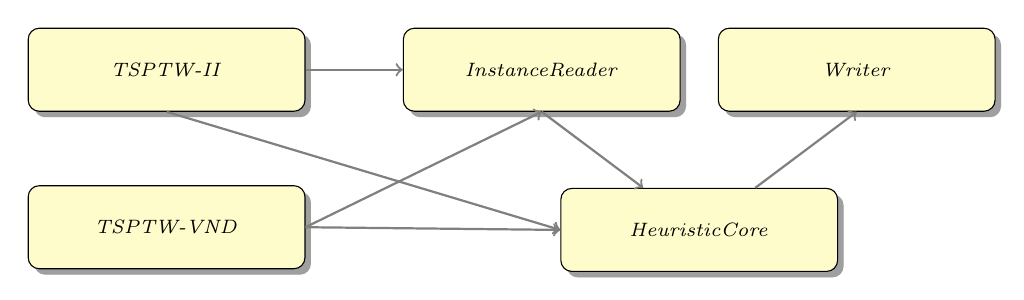
\begin{tikzpicture}[transform shape]
 
  % Draw diagram elements
  
  \path \component {1}{HeuristicCore};
  \path (p1.north)+(-2.0,+1.5) \component{2}{InstanceReader};
  \path (p1.north)+(+2.0,+1.5) \component{3}{Writer};
  \path (p2.west)+(-3.0,0.0) \component{4}{TSPTW-II};
  \path (p2.west)+(-3.0,-2.0) \component{5}{TSPTW-VND}; 
     
  % Draw arrows between elements
  \path [line] (p2.south) -> node [above] {} (p1);
  \path [line] (p1) -> node [above, midway] {} (p3.south);
  \path [line] (p4.east) -> node [above] {} (p2.west);
  \path [line] (p5.east) -> node [above] {} (p2.south);
  \path [line] (p4.south) -> node [above] {} (p1.west);
  \path [line] (p5.east) -> node [above] {} (p1.west);
  
  %\backgroundSquare{p1}{p1}{p3}{p3}{Presentation}

 \end{tikzpicture}
 \captionof{figure}{Simulation Code Structure}
\end{center}

The names of the nodes corresponds to those of the implementation (.cpp) and header files for the corresponding classes.
In addition to these, a class to represent the time windows (TimeWindow.h) and another one to represent the candidate solution as
a user defined data type (CandidateSolution.\{h,cpp\}) have been implemented.


\subsection{How to compile the program?}
The software was developed in C++98 under Linux (Debian Wheezy), using the GNU g++ (Debian 4.7.2-5) 4.7.2 compiler and tested in this environment. 
The software is distributed as a compressed tar file, containing both the source code (in the \verb|src| folder) and the scripts and instances (in the \verb|bin| and \verb|bin\instances| respectively).
To install the program, first obtain the file TSPTW.V1.0.tar.gz. 

Unzip the file by typing:

\begin{center}
\begin{verbatim}
gunzip TSPTW.V1.0.tar.gz
\end{verbatim}
\end{center}

and then unpack it by typing:

\begin{center}
\begin{verbatim}
tar -xvf TSPTW.V1.0.tar
\end{verbatim}
\end{center}

The software will be extracted in a new folder TSPTW.V1.0 

Finally, by launching
\begin{center}
\begin{verbatim}
make all
\end{verbatim}
\end{center}

the Makefile will trigger the compilation of the files,
producing the executables 'TSPTW-II' and 'TSPTW-VND" in the \verb|bin| folder.

\textbf{Note:} The code is written in C++98. Hence, the code should be
reasonable portable to other Operating Systems than Linux or Unix.

\subsection{How to run the program?}

Once the program has been compiled, two separate executable files,
corresponding to the different kind of metaheuristic (i.e. Iterative Improvement
and Variable Neighborhood Descent) can be either launched directly via the command line
interface or using the bash script to launch.

The design choice to separate the two different kind of metaheuristic is made in order to limit the number of command line parameters to be given as input to the program.

\subsubsection{Command-line execution}
By launching\footnote{The squared-bracket notation implies that the formal parameters to the script have to be substituted by their actual value.}:
\begin{center}
\begin{verbatim}
./TSPTW-II [PARAMETERS] -i [INPUT_FILE] -s [SEEDS_FILE]
\end{verbatim}
\begin{verbatim}
./TSPTW-VND [PARAMETERS] -i [INPUT_FILE] -s [SEEDS_FILE]
\end{verbatim}
\end{center}

one can display the information about the meaning of the different options that can be given as input to the program.

Additional information concerning the usage of the program can be found in the README file.

The only mandatory options are "-i, --input" and "-s,-seeds", since
without these components will not be possible to execute the simulation.

The argument to the input option must contain the full path to the instance file.

The seeds file must contain a number of seeds at least equal to the number of
runs required, one seed per line without any additional information.

The options controlling the same parameters are mutually exclusive, with that
meaning that only one option must be selected in order to run the program.
If multiple options for the same parameter are chosen, the program will not
run.

\paragraph{TSPTW-II}
\begin{tabular}{|l|c|}
\hline
\textbf{Parameter}	&	\textbf{Mutually exclusive options} \\ \hline
Initial solution & -d,--random , -h,--heuristic \\ \hline
Neighborhood type &-t,--transpose , -e,--exchange , -n,--insert \\ \hline 
Pivoting rule &	-f,--first-imp , -b,--best-imp \\ \hline
\end{tabular}

\paragraph{TSPTW-VND}

\begin{tabular}{|l|c|}
\hline
\textbf{Parameter}	&	\textbf{Mutually exclusive options} \\ \hline
VND algorithm & -t,--standard , -p,--piped \\ \hline
Neighborhood chain & 	-a,--TEI  , -b,--TIE \\ \hline
\end{tabular}

\paragraph{Output}
Every experiment produces a single file:
\begin{itemize}
  \item \textbf{(II)} $[pivoting\_rule].[neighborhood\_type].[INSTANCE\_NAME]$ with $[pivoting\_rule] \in \{first,best\}$ and $[neighborhood\_type] \in \{transpose,exchange,insert\}$ 
  \item \textbf{(VND)} $[vnd\_type].[neighborhood\_chain].[INSTANCE\_NAME]$ with $[vnd\_type] \in \{standard,piped\}$ and $[neighborhood\_type] \in \{tei,tie\}$
\end{itemize} 
				
					 
\textbf{Examples:} \begin{verbatim}
exchange.best.n80w200.004.txt
standard.tei.n80w20.003.txt
\end{verbatim}


The internal structure of the file is the following: \begin{tabular}{|c|c|c|c|}
\hline
\textbf{Seed}	&	\textbf{CV} & \textbf{CpuTime} & \textbf{PRPD} \\ \hline
\end{tabular}

For each run of the algorithm, the program writes in the file, using a tabulation as separator,
the used seed, the number of constraints violations, the cpu runtime and the penalised relative percentage deviation.


\subsubsection{Script execution}
By launching:
\begin{center}
\begin{verbatim}
./launchTSPTW-II.sh [INSTANCE_NAME] [RUNS] [SEEDS_FILE]
\end{verbatim}
\begin{verbatim}
./launchTSPTW-VND.sh [INSTANCE_NAME] [RUNS] [SEEDS_FILE]
\end{verbatim}
\end{center}

The script will:
\begin{enumerate}
  \item Create the files required by the data processing script to write statistics.
  \item Generate a seed file, named [SEEDS\_FILE] containing [RUNS] randomly generated seeds.
  \item Launch the corresponding TSPTW program for [RUNS]  using all the possible combinations of input options.
  \item Wait for the termination of all the previously launched experiment and call the R data processing script
\end{enumerate}

The script assumes that all the instances are located into the instances folder, hence it is only necessary to indicate the instance name, instead of the complete path.

\paragraph{Output}

Each execution of the script will then generate the files:
\begin{itemize}
  \item $[INSTANCE\_NAME]-CpuTime.pdf$ containing the boxplots of the runtime distribution for each algorithm.
  \item $[INSTANCE\_NAME]-PRPD.pdf$ containing the boxplots of the PRPD distribution for each algorithm.
  \item 
        \begin{itemize}
          \item \textbf{(II)} transpose.first, exchange.first, insert.first, transpose.best, exchange.best, insert.best 
          \item \textbf{(VND)} standard.tei, standard.tie, piped.tei, piped.tie
        \end{itemize}
\end{itemize}

The internal structure of the file is the following:

 
\begin{tabular}{|c|c|c|c|}
\hline
\textbf{Instance}	&	\textbf{Infeasible} & \textbf{mean(PRDP)} &	\textbf{mean(CpuTime)} \\ \hline
\end{tabular}

Each line contains the instance name, the percentage of infeasible runs, the mean PRDP and the mean runtime across [RUNS] runs.

%----------------------------------------------------------------------------------------
%	PROBLEM 1
%----------------------------------------------------------------------------------------

% To have just one problem per page, simply put a \clearpage after each problem
\newpage
\begin{homeworkProblem}
\section{Iterative improvement algorithms}
\subsection{Problem statement}
Implement iterative improvement algorithms with:
\begin{itemize}
  \item first-improvement
  \item best-improvement
\end{itemize}
pivoting rule for each of the three neighborhoods: transpose, exchange, and insert. \\
As a starting solution for iterative improvement, consider a random permutation, that is, use the method “Uninformed Random Picking” (see slides of lectures). Bonus points will be awarded for also considering an insertion heuristic as an alternative to random initialization.
\begin{enumerate}
  \item Run the 6 resulting iterative improvement algorithms (all combinations of the two pivoting rules and the
three neighborhoods) on each of the instances. Repeat each run 100 times with different seed for the random
number generator.
\item Compute the following statistics for each of the 6 iterative improvement algorithms and each instance:
\begin{itemize}
  \item Percentage of runs with constraint violations
  \item Mean penalised relative percentage deviation
  \item Mean computation time
\end{itemize} 
\item Produce boxplots of penalised relative percentage deviation and computation time per instance.
\item Determine using statistical tests (in this case, the Wilcoxon test), whether there is a statistically significant difference between the quality of the solutions generated by the different algorithms.
In particular, compare best vs. first-improvement for each neighborhood, and exchange vs. insertion for each pivoting rule.
\end{enumerate}

\subsection{Experiment results}
\subsubsection{n80w20.001}
\begin{center}
\includegraphics[width=0.6\textwidth,keepaspectratio]{{II/n80w20.001/n80w20.001-CpuTime}.pdf}
\captionof{figure}{n80w20.001 - Runtime boxplots for the different iterative improvement algorithms}
\end{center}

\begin{center}
\includegraphics[width=0.6\textwidth,keepaspectratio]{{II/n80w20.001/n80w20.001-PRPD}.pdf}
\captionof{figure}{n80w20.001 - PRPD boxplots for the different iterative improvement algorithms}
\end{center}

\begin{center}
\begin{tabular}{|l|l|}
\hline
\textbf{Test} & \textbf{P-Value} \\
\hline
First vs best - Transpose&9.74631639820544e-18\\
\hline
First vs best - Exchange&2.04966732989559e-17\\
\hline
First vs best - Insert&1.74838327736385e-15\\
\hline
Exchange vs Insert - First&3.95591160889952e-18\\
\hline
Exchange vs Insert - Best&3.9556885406462e-18\\
\hline
\end{tabular}
\captionof{table}{n80w20.001 - Results of Wilcoxon paired signed rank test}
\end{center}

\subsubsection{n80w20.002}
\begin{center}
\includegraphics[width=0.6\textwidth,keepaspectratio]{{II/n80w20.002/n80w20.002-CpuTime}.pdf}
\captionof{figure}{n80w20.002 - Runtime boxplots for the different iterative improvement algorithms}
\end{center}

\begin{center}
\includegraphics[width=0.6\textwidth,keepaspectratio]{{II/n80w20.002/n80w20.002-PRPD}.pdf}
\captionof{figure}{n80w20.002 - PRPD boxplots for the different iterative improvement algorithms}
\end{center}

\begin{center}
\begin{tabular}{|l|l|}
\hline
\textbf{Test} & \textbf{P-Value} \\
\hline
First vs best - Transpose&3.95591160889952e-18\\
\hline
First vs best - Exchange&1.61703099974578e-17\\
\hline
First vs best - Insert&2.39050570998277e-07\\
\hline
Exchange vs Insert - First&3.95591160889952e-18\\
\hline
Exchange vs Insert - Best&3.9556885406462e-18\\
\hline
\end{tabular}
\captionof{table}{n80w20.002 - Results of Wilcoxon paired signed rank test}
\end{center}

\subsubsection{n80w20.003}
\begin{center}
\includegraphics[width=0.6\textwidth,keepaspectratio]{{II/n80w20.003/n80w20.003-CpuTime}.pdf}
\captionof{figure}{n80w20.003 - Runtime boxplots for the different iterative improvement algorithms}
\end{center}

\begin{center}
\includegraphics[width=0.6\textwidth,keepaspectratio]{{II/n80w20.003/n80w20.003-PRPD}.pdf}
\captionof{figure}{n80w20.003 - PRPD boxplots for the different iterative improvement algorithms}
\end{center}

\begin{center}
\begin{tabular}{|l|l|}
\hline
\textbf{Test} & \textbf{P-Value} \\
\hline
First vs best - Transpose&3.95591160889952e-18\\
\hline
First vs best - Exchange&6.21747363653032e-18\\
\hline
First vs best - Insert&6.2952945764779e-08\\
\hline
Exchange vs Insert - First&3.9556885406462e-18\\
\hline
Exchange vs Insert - Best&3.95591160889952e-18\\
\hline
\end{tabular}
\captionof{table}{n80w20.003 - Results of Wilcoxon paired signed rank test}
\end{center}

\subsubsection{n80w20.004}
\begin{center}
\includegraphics[width=0.6\textwidth,keepaspectratio]{{II/n80w20.004/n80w20.004-CpuTime}.pdf}
\captionof{figure}{n80w20.004 - Runtime boxplots for the different iterative improvement algorithms}
\end{center}

\begin{center}
\includegraphics[width=0.6\textwidth,keepaspectratio]{{II/n80w20.004/n80w20.004-PRPD}.pdf}
\captionof{figure}{n80w20.001 - PRPD boxplots for the different iterative improvement algorithms}
\end{center}

\begin{center}
\begin{tabular}{|l|l|}
\hline
\textbf{Test} & \textbf{P-Value} \\
\hline
First vs best - Transpose&4.33123080260219e-18\\
\hline
First vs best - Exchange&1.5356610755813e-16\\
\hline
First vs best - Insert&4.27702026764362e-14\\
\hline
Exchange vs Insert - First&5.59593516960623e-18\\
\hline
Exchange vs Insert - Best&3.95591160889952e-18\\
\hline
\end{tabular}
\captionof{table}{n80w20.004 - Results of Wilcoxon paired signed rank test}
\end{center}

\subsubsection{n80w20.005}
\begin{center}
\includegraphics[width=0.6\textwidth,keepaspectratio]{{II/n80w20.005/n80w20.005-CpuTime}.pdf}
\captionof{figure}{n80w20.005 - Runtime boxplots for the different iterative improvement algorithms}
\end{center}

\begin{center}
\includegraphics[width=0.6\textwidth,keepaspectratio]{{II/n80w20.005/n80w20.005-PRPD}.pdf}
\captionof{figure}{n80w20.005 - PRPD boxplots for the different iterative improvement algorithms}
\end{center}

\begin{center}
\begin{tabular}{|l|l|}
\hline
\textbf{Test} & \textbf{P-Value} \\
\hline
First vs best - Transpose&4.46398542390809e-18\\
\hline
First vs best - Exchange&4.74166029806301e-18\\
\hline
First vs best - Insert&4.0369131744045e-10\\
\hline
Exchange vs Insert - First&4.74166029806301e-18\\
\hline
Exchange vs Insert - Best&3.95591160889952e-18\\
\hline
\end{tabular}
\captionof{table}{n80w20.005 - Results of Wilcoxon paired signed rank test}
\end{center}

\subsubsection{n80w200.001}
\begin{center}
\includegraphics[width=0.6\textwidth,keepaspectratio]{{II/n80w200.001/n80w200.001-CpuTime}.pdf}
\captionof{figure}{n80w200.001 - Runtime boxplots for the different iterative improvement algorithms}
\end{center}

\begin{center}
\includegraphics[width=0.6\textwidth,keepaspectratio]{{II/n80w200.001/n80w200.001-PRPD}.pdf}
\captionof{figure}{n80w200.001 - PRPD boxplots for the different iterative improvement algorithms}
\end{center}

\begin{center}
\begin{tabular}{|l|l|}
\hline
\textbf{Test} & \textbf{P-Value} \\
\hline
First vs best - Transpose&4.07730530936212e-18\\
\hline
First vs best - Exchange&2.17457280454137e-17\\
\hline
First vs best - Insert&3.95591160889952e-18\\
\hline
Exchange vs Insert - First&3.95591160889952e-18\\
\hline
Exchange vs Insert - Best&3.95591160889952e-18\\
\hline
\end{tabular}
\captionof{table}{n80w200.001 - Results of Wilcoxon paired signed rank test}
\end{center}

\subsubsection{n80w200.002}
\begin{center}
\includegraphics[width=0.6\textwidth,keepaspectratio]{{II/n80w200.002/n80w200.002-CpuTime}.pdf}
\captionof{figure}{n80w200.002 - Runtime boxplots for the different iterative improvement algorithms}
\end{center}

\begin{center}
\includegraphics[width=0.6\textwidth,keepaspectratio]{{II/n80w200.002/n80w200.002-PRPD}.pdf}
\captionof{figure}{n80w200.002 - PRPD boxplots for the different iterative improvement algorithms}
\end{center}

\begin{center}
\begin{tabular}{|l|l|}
\hline
\textbf{Test} & \textbf{P-Value} \\
\hline
First vs best - Transpose&5.19043683699158e-18\\
\hline
First vs best - Exchange&4.6720416035814e-17\\
\hline
First vs best - Insert&3.95591160889952e-18\\
\hline
Exchange vs Insert - First&3.95591160889952e-18\\
\hline
Exchange vs Insert - Best&3.95591160889952e-18\\
\hline
\end{tabular}
\captionof{table}{n80w200.002 - Results of Wilcoxon paired signed rank test}
\end{center}

\subsubsection{n80w200.003}
\begin{center}
\includegraphics[width=0.6\textwidth,keepaspectratio]{{II/n80w200.003/n80w200.003-CpuTime}.pdf}
\captionof{figure}{n80w200.003 - Runtime boxplots for the different iterative improvement algorithms}
\end{center}

\begin{center}
\includegraphics[width=0.6\textwidth,keepaspectratio]{{II/n80w200.003/n80w200.003-PRPD}.pdf}
\captionof{figure}{n80w200.003 - PRPD boxplots for the different iterative improvement algorithms}
\end{center}

\begin{center}
\begin{tabular}{|l|l|}
\hline
\textbf{Test} & \textbf{P-Value} \\
\hline
First vs best - Transpose&4.33123080260219e-18\\
\hline
First vs best - Exchange&7.01070639830382e-18\\
\hline
First vs best - Insert&3.95591160889952e-18\\
\hline
Exchange vs Insert - First&3.95591160889952e-18\\
\hline
Exchange vs Insert - Best&3.95591160889952e-18\\
\hline
\end{tabular}
\captionof{table}{n80w200.003 - Results of Wilcoxon paired signed rank test}
\end{center}

\subsubsection{n80w200.004}
\begin{center}
\includegraphics[width=0.6\textwidth,keepaspectratio]{{II/n80w200.004/n80w200.004-CpuTime}.pdf}
\captionof{figure}{n80w200.004 - Runtime boxplots for the different iterative improvement algorithms}
\end{center}

\begin{center}
\includegraphics[width=0.6\textwidth,keepaspectratio]{{II/n80w200.004/n80w200.004-PRPD}.pdf}
\captionof{figure}{n80w200.001 - PRPD boxplots for the different iterative improvement algorithms}
\end{center}

\begin{center}
\begin{tabular}{|l|l|}
\hline
\textbf{Test} & \textbf{P-Value} \\
\hline
First vs best - Transpose&4.33123080260219e-18\\
\hline
First vs best - Exchange&2.4473398426105e-17\\
\hline
First vs best - Insert&3.95591160889952e-18\\
\hline
Exchange vs Insert - First&3.95591160889952e-18\\
\hline
Exchange vs Insert - Best&3.95591160889952e-18\\
\hline
\end{tabular}
\captionof{table}{n80w200.004 - Results of Wilcoxon paired signed rank test}
\end{center}

\subsubsection{n80w200.005}
\begin{center}
\includegraphics[width=0.6\textwidth,keepaspectratio]{{II/n80w200.005/n80w200.005-CpuTime}.pdf}
\captionof{figure}{n80w200.005 - Runtime boxplots for the different iterative improvement algorithms}
\end{center}

\begin{center}
\includegraphics[width=0.6\textwidth,keepaspectratio]{{II/n80w200.005/n80w200.005-PRPD}.pdf}
\captionof{figure}{n80w200.005 - PRPD boxplots for the different iterative improvement algorithms}
\end{center}

\begin{center}
\begin{tabular}{|l|l|}
\hline
\textbf{Test} & \textbf{P-Value} \\
\hline
First vs best - Transpose&4.74166029806301e-18\\
\hline
First vs best - Exchange&1.40854365025687e-16\\
\hline
First vs best - Insert&3.95591160889952e-18\\
\hline
Exchange vs Insert - First&3.95591160889952e-18\\
\hline
Exchange vs Insert - Best&3.95591160889952e-18\\
\hline
\end{tabular}
\captionof{table}{n80w200.005 - Results of Wilcoxon paired signed rank test}
\end{center}

\subsection{Statistics}

\subsubsection{Transpose-First Improvement}
\begin{center}
\begin{tabular}{|l|c|l|l|}
\hline
\textbf{Instance}& \textbf{\% Infeasible} & $\mathbf{\bar{PRDP}}$ &$\mathbf{\bar{Runtime}}$\\
\hline
n80w20.001&1&1229712.6&0.0100035563\\
\hline
n80w20.002&1&1028075.17&0.0095843375\\
\hline
n80w20.003&1&1132968.5&0.0098099452\\
\hline
n80w20.005&1&1010681.79&0.0097989762\\
\hline
n80w20.004&1&1226174.6&0.0094877067\\
\hline
n80w200.001&1&1467634.1&0.0098152878\\
\hline
n80w200.002&1&1504523.7&0.0099101404\\
\hline
n80w200.004&1&1388037.6&0.0098893615\\
\hline
n80w200.003&1&1567210.5&0.0097697727\\
\hline
n80w200.005&1&1644110.9&0.0097550971\\
\hline
\end{tabular}
\captionof{table}{Statistics summary for iterative improvement algorithm with Transpose neighborhood and First Improvement pivoting rule}
\end{center}

\subsubsection{Transpose-Best Improvement}
\begin{center}
\begin{tabular}{|l|c|l|l|}
\hline
\textbf{Instance}& \textbf{\% Infeasible} & $\mathbf{\bar{PRDP}}$ &$\mathbf{\bar{Runtime}}$\\
\hline
n80w20.001&1&1236039.3&0.014545497\\
\hline
n80w20.002&1&1033090.48&0.0145450422\\
\hline
n80w20.003&1&1137758.7&0.014536776\\
\hline
n80w20.005&1&1014818.46&0.014947609\\
\hline
n80w20.004&1&1232996&0.015151286\\
\hline
n80w200.001&1&1476994.8&0.0147534638\\
\hline
n80w200.002&1&1511281&0.014884921\\
\hline
n80w200.004&1&1392023.3&0.0146445173\\
\hline
n80w200.003&1&1575355.5&0.0143582468\\
\hline
n80w200.005&1&1653419.6&0.0150098656\\
\hline
\end{tabular}
\captionof{table}{Statistics summary for iterative improvement algorithm with Transpose neighborhood and Best Improvement pivoting rule}
\end{center}

\subsubsection{Exchange-First Improvement}
\begin{center}
\begin{tabular}{|l|c|l|l|}
\hline
\textbf{Instance}& \textbf{\% Infeasible} & $\mathbf{\bar{PRDP}}$ &$\mathbf{\bar{Runtime}}$\\
\hline
n80w20.001&1&1035718.78&18.390814\\
\hline
n80w20.002&1&884386.3&18.198632\\
\hline
n80w20.003&1&956518.77&18.913801\\
\hline
n80w20.005&1&849054.52&19.043496\\
\hline
n80w20.004&1&1030411.56&19.660314\\
\hline
n80w200.001&1&661322.18&23.117446\\
\hline
n80w200.002&1&813339.6&22.552976\\
\hline
n80w200.004&1&679489.06&22.068859\\
\hline
n80w200.003&1&697450.03&24.338257\\
\hline
n80w200.005&1&760027.65&22.348975\\
\hline
\end{tabular}
\captionof{table}{Statistics summary for iterative improvement algorithm with Exchange neighborhood and First Improvement pivoting rule}
\end{center}

\subsubsection{Exchange-Best Improvement}
\begin{center}
\begin{tabular}{|l|c|l|l|}
\hline
\textbf{Instance}& \textbf{\% Infeasible} & $\mathbf{\bar{PRDP}}$ &$\mathbf{\bar{Runtime}}$\\
\hline
n80w20.001&1&1086217.68&13.091453\\
\hline
n80w20.002&1&901762.05&13.365301\\
\hline
n80w20.003&1&1017243.86&13.267128\\
\hline
n80w20.005&1&895720.53&13.5824245\\
\hline
n80w20.004&1&1084080.4&14.189582\\
\hline
n80w200.001&1&1022433.76&16.418229\\
\hline
n80w200.002&1&1075649.94&16.028712\\
\hline
n80w200.004&1&994703.67&15.518766\\
\hline
n80w200.003&1&1094460.9&16.16696\\
\hline
n80w200.005&1&1110949.86&16.566802\\
\hline
\end{tabular}
\captionof{table}{Statistics summary for iterative improvement algorithm with Exchange neighborhood and Best Improvement pivoting rule}
\end{center}

\subsubsection{Insert-First Improvement}
\begin{center}
\begin{tabular}{|l|c|l|l|}
\hline
\textbf{Instance}& \textbf{\% Infeasible} & $\mathbf{\bar{PRDP}}$ &$\mathbf{\bar{Runtime}}$\\
\hline
n80w20.001&0.65&16070.27322082&25.88279\\
\hline
n80w20.002&0.83&11803.71462682&28.509938\\
\hline
n80w20.003&0.83&21587.617&28.579453\\
\hline
n80w20.005&0.32&4945.642107&28.672083\\
\hline
n80w20.004&0.49&10894.01867489&28.474429\\
\hline
n80w200.001&0.22&6119.9927045&59.544212\\
\hline
n80w200.002&0&11.2561521&64.580306\\
\hline
n80w200.004&0.11&3049.80805246&63.942238\\
\hline
n80w200.003&0.01&437.87774695&63.687806\\
\hline
n80w200.005&0.01&464.62990671&66.084369\\
\hline

\end{tabular}
\captionof{table}{Statistics summary for iterative improvement algorithm with Insert neighborhood and First Improvement pivoting rule}
\end{center}

\subsubsection{Insert-Best Improvement}
\begin{center}
\begin{tabular}{|l|c|l|l|}
\hline
\textbf{Instance}& \textbf{\% Infeasible} & $\mathbf{\bar{PRDP}}$ &$\mathbf{\bar{Runtime}}$\\
\hline
n80w20.001&0.56&14772.44442862&28.769951\\
\hline
n80w20.002&0.84&16009.51797952&30.159812\\
\hline
n80w20.003&0.89&26984.256&30.197019\\
\hline
n80w20.005&0.52&10159.3062354&30.776906\\
\hline
n80w20.004&0.59&18861.32619536&31.013\\
\hline
n80w200.001&0.37&21195.2243605&33.031965\\
\hline
n80w200.002&0&13.2172159&33.011011\\
\hline
n80w200.004&0.42&23019.4946845&34.123681\\
\hline
n80w200.003&0.12&7740.06242146&34.080592\\
\hline
n80w200.005&0.07&2516.0079072&33.450537\\
\hline
\end{tabular}
\captionof{table}{Statistics summary for iterative improvement algorithm with Insert neighborhood and Best Improvement pivoting rule}
\end{center}

\end{homeworkProblem}		

%----------------------------------------------------------------------------------------
%	PROBLEM 1
%----------------------------------------------------------------------------------------

% To have just one problem per page, simply put a \clearpage after each problem
\newpage
\begin{homeworkProblem}
\section{Variable neighborhood descent algorithms}
\subsection{Problem statement}
Implement both a standard and piped variable neighborhood descent (VND) algorithm (concatenation of the underlying iterative improvement algorithms; see lecture slides). Consider the two possible (reasonable) orderings of
the iterative improvement algorithms (indicated by the neighborhood relation they use):
\begin{itemize}
  \item transpose, exchange, insert
  \item transpose, insert, exchange 
\end{itemize}
Implement the 4 VND algorithms (all combinations of standard and piped and the two neighborhood orders) using first-improvement and random initialization.

\subsection{Introduction}
An Iterative Improvement algorithm generally starts from a candidate solution, which can be either generated randomly or using an heuristic, and improves the evaluation of the solution at each step by modifying the solution structure , until a local optimum is reached.

In the previous problem, I considered different kinds of 2-opt neighborhood, and different pivoting rules.

This means that, at each step, a new solution is constructed from the current best by modifying only two solution components (with Transpose,Exchange or Insert operations) and only the first/best improving solution will become the new best soluion.

The main limitation of such kind of algorithms is that they tend to get stuck in solutions that are locally optimum but not globally.

Provided that:
\begin{itemize}
\item A global optimum is optimal with respect to any kind of neighborhood. 
\item A solution that is locally optimal with respect to a neighborhood may not be optimal with respect to other kinds of neighborhood
\end{itemize}
by dynamically changing the neighborhood type an algorithm is able to escape local optima.

This section will analyse the results of the execution of two variable neighborhood descent algorithm, based on the previously analyzed iterative improvement algorithms :
\begin{itemize}
\item \textbf{Standard Variable Neighborhood Descent} (i.e. Changing neighborhood when a local optimum is encoutered, until the neighborhood chain is terminated and going back to the smallest neighborhood every time the local optimum is escaped.)
\item \textbf{Piped Variable Neighborhood Descent} (i.e. Using the locally optimum solution found using one neighborhood type in the chain as the initial solution for the following type.)
\end{itemize}
The same metrics as in \ref{subsec:metric} will be used to evaluate the algorithms.

\subsection{Experiment results}
\subsubsection{n80w20.001}
\begin{center}
\includegraphics[width=0.6\textwidth,keepaspectratio]{{VND/n80w20.001/n80w20.001-CpuTime}.pdf}
\captionof{figure}{n80w20.001 - Runtime boxplots for the different variable neighborhood descent algorithms}
\end{center}

\begin{center}
\includegraphics[width=0.6\textwidth,keepaspectratio]{{VND/n80w20.001/n80w20.001-PRPD}.pdf}
\captionof{figure}{n80w20.001 - PRPD boxplots for the different variable neighborhood descent algorithms}
\end{center}

\begin{center}
\begin{tabular}{|l|l|}
\hline
\textbf{Test} & \textbf{P-Value} \\
\hline
Tei vs Tie - Standard&3.95591160889952e-18\\
\hline
Tei vs Tie - Piped&3.9556885406462e-18\\
\hline
Standard vs Piped - Tei&3.95591160889952e-18\\
\hline
Standard vs Piped - Tie&3.95591160889952e-18\\
\hline
\end{tabular}
\captionof{table}{n80w20.001 - Results of Wilcoxon paired signed rank test}
\label{tab:w.11}
\end{center}

\subsubsection{n80w20.002}
\begin{center}
\includegraphics[width=0.6\textwidth,keepaspectratio]{{VND/n80w20.002/n80w20.002-CpuTime}.pdf}
\captionof{figure}{n80w20.002 - Runtime boxplots for the different variable neighborhood descent algorithms}
\end{center}

\begin{center}
\includegraphics[width=0.6\textwidth,keepaspectratio]{{VND/n80w20.002/n80w20.002-PRPD}.pdf}
\captionof{figure}{n80w20.002 - PRPD boxplots for the different variable neighborhood descent algorithms}
\end{center}

\begin{center}
\begin{tabular}{|l|l|}
\hline
\textbf{Test} & \textbf{P-Value} \\
\hline
Tei vs Tie - Standard&3.9556885406462e-18\\
\hline
Tei vs Tie - Piped&3.95591160889952e-18\\
\hline
Standard vs Piped - Tei&3.95591160889952e-18\\
\hline
Standard vs Piped - Tie&3.95591160889952e-18\\
\hline
\end{tabular}
\captionof{table}{n80w20.002 - Results of Wilcoxon paired signed rank test}
\label{tab:w.12}
\end{center}

\subsubsection{n80w20.003}
\begin{center}
\includegraphics[width=0.6\textwidth,keepaspectratio]{{VND/n80w20.003/n80w20.003-CpuTime}.pdf}
\captionof{figure}{n80w20.003 - Runtime boxplots for the different variable neighborhood descent algorithms}
\end{center}

\begin{center}
\includegraphics[width=0.6\textwidth,keepaspectratio]{{VND/n80w20.003/n80w20.003-PRPD}.pdf}
\captionof{figure}{n80w20.003 - PRPD boxplots for the different variable neighborhood descent algorithms}
\end{center}

\begin{center}
\begin{tabular}{|l|l|}
\hline
\textbf{Test} & \textbf{P-Value} \\
\hline
Tei vs Tie - Standard&3.9552424399092e-18\\
\hline
Tei vs Tie - Piped&3.95591160889952e-18\\
\hline
Standard vs Piped - Tei&3.95591160889952e-18\\
\hline
Standard vs Piped - Tie&3.95591160889952e-18\\
\hline
\end{tabular}
\captionof{table}{n80w20.003 - Results of Wilcoxon paired signed rank test}
\label{tab:w.13}
\end{center}

\subsubsection{n80w20.004}
\begin{center}
\includegraphics[width=0.6\textwidth,keepaspectratio]{{VND/n80w20.004/n80w20.004-CpuTime}.pdf}
\captionof{figure}{n80w20.004 - Runtime boxplots for the different variable neighborhood descent algorithms}
\end{center}

\begin{center}
\includegraphics[width=0.6\textwidth,keepaspectratio]{{VND/n80w20.004/n80w20.004-PRPD}.pdf}
\captionof{figure}{n80w20.004 - PRPD boxplots for the different variable neighborhood descent algorithms}
\end{center}

\begin{center}
\begin{tabular}{|l|l|}
\hline
\textbf{Test} & \textbf{P-Value} \\
\hline
Tei vs Tie - Standard&3.95591160889952e-18\\
\hline
Tei vs Tie - Piped&3.95591160889952e-18\\
\hline
Standard vs Piped - Tei&3.95591160889952e-18\\
\hline
Standard vs Piped - Tie&3.95591160889952e-18\\
\hline
\end{tabular}
\captionof{table}{n80w20.004 - Results of Wilcoxon paired signed rank test}
\label{tab:w.14}
\end{center}

\subsubsection{n80w20.005}
\begin{center}
\includegraphics[width=0.6\textwidth,keepaspectratio]{{VND/n80w20.005/n80w20.005-CpuTime}.pdf}
\captionof{figure}{n80w20.005 - Runtime boxplots for the different variable neighborhood descent algorithms}
\end{center}

\begin{center}
\includegraphics[width=0.6\textwidth,keepaspectratio]{{VND/n80w20.005/n80w20.005-PRPD}.pdf}
\captionof{figure}{n80w20.001 - PRPD boxplots for the different variable neighborhood descent algorithms}
\end{center}

\begin{center}
\begin{tabular}{|l|l|}
\hline
\textbf{Test} & \textbf{P-Value} \\
\hline
Tei vs Tie - Standard&3.95591160889952e-18\\
\hline
Tei vs Tie - Piped&3.95591160889952e-18\\
\hline
Standard vs Piped - Tei&3.95591160889952e-18\\
\hline
Standard vs Piped - Tie&3.95591160889952e-18\\
\hline
\end{tabular}
\captionof{table}{n80w20.005 - Results of Wilcoxon paired signed rank test}
\label{tab:w.15}
\end{center}

\subsubsection{n80w200.001}
\begin{center}
\includegraphics[width=0.6\textwidth,keepaspectratio]{{VND/n80w200.001/n80w200.001-CpuTime}.pdf}
\captionof{figure}{n80w200.001 - Runtime boxplots for the different variable neighborhood descent algorithms}
\end{center}

\begin{center}
\includegraphics[width=0.6\textwidth,keepaspectratio]{{VND/n80w200.001/n80w200.001-PRPD}.pdf}
\captionof{figure}{n80w200.001 - PRPD boxplots for the different variable neighborhood descent algorithms}
\end{center}

\begin{center}
\begin{tabular}{|l|l|}
\hline
\textbf{Test} & \textbf{P-Value} \\
\hline
Tei vs Tie - Standard&4.07730530936212e-18\\
\hline
Tei vs Tie - Piped&2.92094064174088e-17\\
\hline
Standard vs Piped - Tei&2.72456795287507e-16\\
\hline
Standard vs Piped - Tie&3.95591160889952e-18\\
\hline
\end{tabular}
\captionof{table}{n80w200.001 - Results of Wilcoxon paired signed rank test}
\label{tab:w.16}
\end{center}

\subsubsection{n80w200.002}
\begin{center}
\includegraphics[width=0.6\textwidth,keepaspectratio]{{VND/n80w200.002/n80w200.002-CpuTime}.pdf}
\captionof{figure}{n80w200.002 - Runtime boxplots for the different variable neighborhood descent algorithms}
\end{center}

\begin{center}
\includegraphics[width=0.6\textwidth,keepaspectratio]{{VND/n80w200.002/n80w200.002-PRPD}.pdf}
\captionof{figure}{n80w200.002 - PRPD boxplots for the different variable neighborhood descent algorithms}
\end{center}

\begin{center}
\begin{tabular}{|l|l|}
\hline
\textbf{Test} & \textbf{P-Value} \\
\hline
Tei vs Tie - Standard&3.95591160889952e-18\\
\hline
Tei vs Tie - Piped&1.52379449675399e-17\\
\hline
Standard vs Piped - Tei&1.74838327736385e-15\\
\hline
Standard vs Piped - Tie&3.95591160889952e-18\\
\hline
\end{tabular}
\captionof{table}{n80w200.002 - Results of Wilcoxon paired signed rank test}
\label{tab:w.17}
\end{center}

\subsubsection{n80w200.003}
\begin{center}
\includegraphics[width=0.6\textwidth,keepaspectratio]{{VND/n80w200.003/n80w200.003-CpuTime}.pdf}
\captionof{figure}{n80w200.003 - Runtime boxplots for the different variable neighborhood descent algorithms}
\end{center}

\begin{center}
\includegraphics[width=0.6\textwidth,keepaspectratio]{{VND/n80w200.003/n80w200.003-PRPD}.pdf}
\captionof{figure}{n80w200.003 - PRPD boxplots for the different variable neighborhood descent algorithms}
\end{center}

\begin{center}
\begin{tabular}{|l|l|}
\hline
\textbf{Test} & \textbf{P-Value} \\
\hline
Tei vs Tie - Standard&2.04955667109233e-17\\
\hline
Tei vs Tie - Piped&2.59611565456869e-17\\
\hline
Standard vs Piped - Tei&1.50422804122146e-07\\
\hline
Standard vs Piped - Tie&3.95591160889952e-18\\
\hline
\end{tabular}
\captionof{table}{n80w200.003 - Results of Wilcoxon paired signed rank test}
\label{tab:w.18}
\end{center}

\subsubsection{n80w200.004}
\begin{center}
\includegraphics[width=0.6\textwidth,keepaspectratio]{{VND/n80w200.004/n80w200.004-CpuTime}.pdf}
\captionof{figure}{n80w200.004 - Runtime boxplots for the different variable neighborhood descent algorithms}
\end{center}

\begin{center}
\includegraphics[width=0.6\textwidth,keepaspectratio]{{VND/n80w200.004/n80w200.004-PRPD}.pdf}
\captionof{figure}{n80w200.004 - PRPD boxplots for the different variable neighborhood descent algorithms}
\end{center}

\begin{center}
\begin{tabular}{|l|l|}
\hline
\textbf{Test} & \textbf{P-Value} \\
\hline
Tei vs Tie - Standard&4.07730530936212e-18\\
\hline
Tei vs Tie - Piped&4.29577057320019e-16\\
\hline
Standard vs Piped - Tei&5.3075517052254e-11\\
\hline
Standard vs Piped - Tie&3.95591160889952e-18\\
\hline
\end{tabular}
\captionof{table}{n80w200.004 - Results of Wilcoxon paired signed rank test}
\label{tab:w.19}
\end{center}

\subsubsection{n80w200.005}
\begin{center}
\includegraphics[width=0.6\textwidth,keepaspectratio]{{VND/n80w200.005/n80w200.005-CpuTime}.pdf}
\captionof{figure}{n80w200.005 - Runtime boxplots for the different variable neighborhood descent algorithms}
\end{center}

\begin{center}
\includegraphics[width=0.6\textwidth,keepaspectratio]{{VND/n80w200.005/n80w200.005-PRPD}.pdf}
\captionof{figure}{n80w200.001 - PRPD boxplots for the different variable neighborhood descent algorithms}
\end{center}

\begin{center}
\begin{tabular}{|l|l|}
\hline
\textbf{Test} & \textbf{P-Value} \\
\hline
Tei vs Tie - Standard&1.39380002081336e-17\\
\hline
Tei vs Tie - Piped&4.07730530936212e-18\\
\hline
Standard vs Piped - Tei&3.72316935219101e-06\\
\hline
Standard vs Piped - Tie&3.95591160889952e-18\\
\hline
\end{tabular}
\captionof{table}{n80w200.001 - Results of Wilcoxon paired signed rank test}
\label{tab:w.20}
\end{center}

\subsection{Statistics}
\subsubsection{Standard-Transpose-Exchange-Insert}
\begin{center}
\begin{tabular}{|l|c|l|l|}
\hline
\textbf{Instance}& \textbf{\% Infeasible} & $\mathbf{\bar{PRDP}}$ &$\mathbf{\bar{Runtime}}$\\
\hline
n80w20.001&0.71&14772.04644164&50.611339\\
\hline
n80w20.002&0.88&12888.542&50.727053\\
\hline
n80w20.003&0.92&19936.872&50.820348\\
\hline
n80w20.004&0.62&17234.94260984&50.049484\\
\hline
n80w20.005&0.94&12564.0560428&50.269182\\
\hline
n80w200.001&0.28&11212.97389136&49.151249\\
\hline
n80w200.002&0.03&629.5853274&51.433949\\
\hline
n80w200.003&0.07&1511.56628539&49.082085\\
\hline
n80w200.004&0.16&4193.4817209&49.662512\\
\hline
n80w200.005&0.01&466.6729061&46.701953\\
\hline
\end{tabular}
\captionof{table}{Statistics summary for variable neighborhood descent algorithm with Transpose-Exchange-Insert neighborhood chain and Standard VND type}
\label{tab:s.tei}
\end{center}

\subsubsection{Standard-Transpose-Insert-Exchange}
\begin{center}
\begin{tabular}{|l|c|l|l|}
\hline
\textbf{Instance}& \textbf{\% Infeasible} & $\mathbf{\bar{PRDP}}$ &$\mathbf{\bar{Runtime}}$\\
\hline
n80w20.001&0.54&10874.77632472&15.268454\\
\hline
n80w20.002&0.62&8411.724&15.386641\\
\hline
n80w20.003&0.44&7645.295&15.638153\\
\hline
n80w20.004&0.39&7153.68881324&15.980347\\
\hline
n80w20.005&0.25&3475.2731712&15.55767\\
\hline
n80w200.001&0.16&4898.3227617&33.424555\\
\hline
n80w200.002&0&11.0430351&32.198479\\
\hline
n80w200.003&0.05&1082.1460308&34.345522\\
\hline
n80w200.004&0.28&7804.19186258&32.583152\\
\hline
n80w200.005&0&10.20227353&34.501294\\
\hline
\end{tabular}
\captionof{table}{Statistics summary for variable neighborhood descent algorithm with Transpose-Insert-Exchange neighborhood chain and Standard VND type}
\label{tab:s.tie}
\end{center}

\subsubsection{Piped-Transpose-Exchange-Insert}
\begin{center}
\begin{tabular}{|l|c|l|l|}
\hline
\textbf{Instance}& \textbf{\% Infeasible} & $\mathbf{\bar{PRDP}}$ &$\mathbf{\bar{Runtime}}$\\
\hline
n80w20.001&0.59&12336.84228578&35.694416\\
\hline
n80w20.002&0.94&15603.0142035&36.212393\\
\hline
n80w20.003&0.83&19338.924&34.821217\\
\hline
n80w20.004&0.55&13170.33921962&36.438959\\
\hline
n80w20.005&0.45&6683.336214&36.202891\\
\hline
n80w200.001&0.19&5104.3621015&40.772642\\
\hline
n80w200.002&0.01&218.8179842&44.241593\\
\hline
n80w200.003&0.06&2584.90674231&44.725066\\
\hline
n80w200.004&0.17&3430.64506042&43.760992\\
\hline
n80w200.005&0.02&693.0136326&42.646023\\
\hline
\end{tabular}
\captionof{table}{Statistics summary for variable neighborhood descent algorithm with Transpose-Exchange-Insert neighborhood chain and Piped VND type}
\label{tab:p.tei}
\end{center}

\subsubsection{Piped-Transpose-Insert-Exchange}
\begin{center}
\begin{tabular}{|l|c|l|l|}
\hline
\textbf{Instance}& \textbf{\% Infeasible} & $\mathbf{\bar{PRDP}}$ &$\mathbf{\bar{Runtime}}$\\
\hline
n80w20.001&0.68&16393.81210394&24.788225\\
\hline
n80w20.002&0.81&11667.654&25.902581\\
\hline
n80w20.003&0.84&20537.669&26.442309\\
\hline
n80w20.004&0.46&8779.79314651&26.424231\\
\hline
n80w20.005&0.24&3876.3661498&26.511156\\
\hline
n80w200.001&0.21&5917.0312803&52.302366\\
\hline
n80w200.002&0.01&626.0983757&56.238843\\
\hline
n80w200.003&0.04&867.92563269&58.498874\\
\hline
n80w200.004&0.28&6281.58944822&55.867038\\
\hline
n80w200.005&0.01&236.8657243&58.331595\\
\hline
\end{tabular}
\captionof{table}{Statistics summary for variable neighborhood descent algorithm with Transpose-Insert-Exchange neighborhood chain and Piped VND type}
\label{tab:p.tie}
\end{center}

\subsection{Results discussion}
By looking at tables \ref{tab:s.tei}, \ref{tab:s.tie}, \ref{tab:p.tei}, \ref{tab:p.tie} one can see that:
\begin{itemize}

\item For some instances (e.g. $n80w20.002$,$n80w20.003$) the algorithm are not able to converge to a feasible solution, as shown in the corresponding boxplots, since the PRPD distribution is centered around 12000-15000, thus indicating the presence of at least 1 constraint violations in most of the cases.

\item For some other instances (e.g. $n80w20.004$,$n80w20.005$) the algorithms are able to converge to feasible solutions and to the best-known one, but having a right-skewed distribution towards higher values of PRPD.

\item For the remaining instances, except for some outlier values, the algorithms are able to converge to the best-known solution in most of the runs , even though the average PRPD is not closer to 0. This is due to the fact that the mean of a distribution is sensible to outliers and the penalisation for a constraint violations is extremely high when compared to the mean value.
      
\item The algorithm ordering in terms of runtimes is $s.tie < p.tie < p.tei < s.tei$ for the  $n80w20.X$ instances while $s.tie < p.tei < s.tei < p.tie$ for $n80w200.X$ ones. The choice to explore the Insert Neighborhood before the Exchange one allows to reduce the computation time for the $n80w20.X$ instances, with a similar solution quality.

\item The algorithms are more effective on the $n80w200.X$ instances then the $n80w20.X$ once, since they have a lower percentage of infeasible runs and a lower PRPD.

\item The standard variable neighborhood descent with Transpose-Insert-Exchange neighborhood chain (s.tie) outperforms all the other algorithms in terms of solution quality and runtime.

\item Tables \ref{tab:w.11}, \ref{tab:w.12}, \ref{tab:w.13}, \ref{tab:w.14}, \ref{tab:w.15}, \ref{tab:w.16}, \ref{tab:w.17}, \ref{tab:w.18}, \ref{tab:w.19}, \ref{tab:w.20} contain, in any case, p-values considerably smaller than the significance level ($\alpha=0.05$). 

This implies that the null hypothesis corresponding to the equality of the median values of the differences of the two distributions can be rejected, hence assessing the existence of a statistically significant difference among the solution quality generated by analyzed algorithms.

\item By looking at the Cpu time, one can see that the instances \emph{n80w20.X} have generally lower runtimes than the \emph{n80w200.X} ones. They can then be considered, with respect to the variable neighborhood descent algorithms, simpler (quickier to solve) instances with respect to the latter.

\end{itemize}

\end{homeworkProblem}


% \subsection{Simulation code}


% \subsubsection{Simulation execution module}

% \paragraph{Description}
% This module contains all the necessary code to actually perform the simulation of the moran Process, namely the functions:
% \begin{itemize}
% \item \emph{simulationStepRelativeFitness()}
% \item \emph{updateFitness()}
% \end{itemize}

% The simulation module obtains the preprocessed data from the corresponding module, then, for each of the 36 simulation:
% \begin{enumerate}
% \item Generates a population of $N$ individuals, $i$ of which of A-type.
% \item Computes the initial fitness $f_A$ and $f_B$ of the population.
% \item Performs \emph{ITERATION} runs of maximum $10*N$ simulation step each.
% \item Calls the postprocessing module to produce a syntactically correct \LaTeX  file.
% \end{enumerate}

% \subparagraph{updateFitness()}
% The expected payoff of A-type players, as in \cite{Taylor2004}, is determined as follows: 
% \begin{equation}
% p_A = a\cdot(i - 1) + b\cdot(N - i)
% \end{equation}
% while, for B-type players:
% \begin{equation}
% p_B = c\cdot i + d(N - i - 1)
% \end{equation}
% The fitness of each type of players is then determined according to \cite{Traulsen2010}:
% \begin{equation}
% \begin{array}{c}
% f_A = 1-w+w\cdot p_A\\
% f_B = 1-w+w\cdot p_B\\
% \end{array}
% \end{equation}
% The intensity of selection $w \in [0,1]$ determines the relevance of the payoff in the computation of the fitness.\\
% For the simulation it is chosen to be equal to $0.5$ in order neither to perform an individual duplication depending solely on the payoff ($w=1$) nor to have a completely random selection($w=0$).

% \paragraph{simulationStepRelativeFitness()}
% In each simulation step, an individual is selected at random to be eliminated and replaced by a copy of another existing individual in the population.\\
% The duplication of an A-type individual occurs with a probability which is fitness dependant, as in \cite{Taylor2004}:
% \begin{equation}
% p_{D_A} = \frac{i \cdot f_A}{i \cdot f_A + (N-i)\cdot f_B}
% \end{equation}
% The number of A-type players is then adjusted according to the outcome of the probabilistic duplication.

% %\pyscript{./Simulation/moranProcess}{}

% \subsubsection{Output post-processing module}
% At the end of each simulation, the functions of the \LaTeX post-processing module are called to produce the files, used to typeset the simulation results.\\
% %\pyscript{./Simulation/latexReport}{}

% \clearpage


% \end{homeworkProblem}

% % \begin{homeworkProblem}
% % \section{Analysis of simulation results}
% % \label{sec:simres}
% % The following section presents the results of the simulation performed by executing the Python script.\\
% % One should remember, that the population is initialized with $1$ A-Type individual and $N-1$ B-Type individual.\\
% % At the end of every section, an overview of the results is shown stating:
% % \begin{itemize}
% % \item \textbf{Coherent}:
% % 	\begin{itemize}
% % 	\item \cmark - Whenever the expected result for an infinite population agrees with the results of the simulation.
% % 	\item \xmark - If, due to some stochastic effect, the outcome of the simulation is different from what is expected.
% % 	\end{itemize}
% % \item\textbf{Stable against invasion}:
% % 	\begin{itemize}
% % 	\item \cmark - Whenever the number of A-Type individuals converges to 0 at the end of the simulation.
% % 	\item \xmark - If, either the invasion of a single A-Type individual can cause the extinction of B-Type players ($x_A=N$) or the stable state at the end of the simulation has a non null number of A-Type agents ($x_A=x^*$).
% % 	\end{itemize}
% % \end{itemize}
% % It should be remarked that the outcome of the simulation is chosen to be the outcome having the greatest occurrence for each simulation.\\
% % Whenever there are other outcomes with a non negligible number of occurrences ($o_i>10^3$), the theoretical results and the experimental results are discordant. 
% % %\input{simulationResults}

% % \end{homeworkProblem}


% %----------------------------------------------------------------------------------------
% %	PROBLEM 2
% %----------------------------------------------------------------------------------------
% \begin{homeworkProblem}

% \section{Variable Neighborhood Descent algorithms }
% \subsection{Problem statement}
% \subsubsection{Game description}
% In  a  dictator  game  two  players  are  interacting.\\   
% The  first  player  (also  called  the   proposer)  decides  on  how  some  endowment  is  split  between  the  players. \\
% The   second  player  simply  receives  his  part  of  the  split. \\     
% So  the  role  of  the  receiver  is   completely  passive,  no  decisions  have  to  be  taken  when  a  player  fulfills  that  role.
% \\   We  assume  here  that  the  proposer  can  select  between  three  actions:    a  selfish,  a   fair   and   an   altruistic   split. \\
% In   the   selfish   split,   she   keeps   the   majority   of   the   endowment  and  in  the  altruistic  action  she  hands  over  almost  all  the  endowment   to  the  receiver. \\ 
% In  the  fair  case,  she  splits  the  endowment  in  an  equal  manner. \\        
% As  opposed  to  the  normal  Dictator  Game,  we  will  now  assume  here  that  in  this   game,  before  the  dictator  proposes  a  split,  the  player  needs  to  decide  whether  he   or  she  wants  to  play  the  game.  So  now  the  player  has  two  actions  “play”  or    “not   play”. \\
% If  the  receiver  decides  to  play,  the  proposer  simply  decides  the  split.  If  the   receiver  decides  not  to  play  both  get  zero  payoff.     

% \subsubsection{Part I}
% \begin{enumerate}
% \item Draw  the  Extensive  Form  Game  that  corresponds  and  report  the  Subgame  Perfect  equilibrium. 
% \item Create   the   Strategic   Form   of   this   game   and   determine   the   Nash  Equilibrium  of  this  game. 
% \end{enumerate}


% \subsubsection{Part II}
% The  game  is  clearly  not  symmetric. Yet  we  can  make  it  so. \\    We  need  to  assume   that  a  strategy  takes  the  role  of  the  player  into  account. \\
% When  two  players  meet   their  role  is  randomly  assigned.  A  pure  strategy  of  for  each  of  these  players  can   be  written  as  ‘xy’  which  means  ‘if  I  am  the  proposer  I  play  x  if  I  am  the  receiver  I   play  y’,  where  the  ‘x’  is  either  ‘selfish  split’  (S),  ‘altruistic  split’  (A)    or  ‘Fair  split’   (F)  and  the  ‘y’  is  either  ‘Play  (P)  or    ‘Don’t  play’  (N).\\    
% The  payoff  they  receive  is   the  mean  of  the  payoffs  for  both  choices.     
% \begin{enumerate}
% \item How  many  pure  strategies  are  there  for  each  player? 
% \item Write   down   the   normal   form   and   determine   the   Nash   equilibria   of   this  game. 
% \end{enumerate}

% \subsection{Proposed solution}
% \subsubsection{Question 1}
% \paragraph{Modeling assumptions}
% \label{par:modeling}
% The original Dictator game is formally a two-players degenerate game, in the sense that the outcome of the game does not depend on the choices made by all the players in the game, with the second player having a completely passive role.\\
% The proposed modification makes the problem a proper sequential game, thus allowing one to represent it using the extensive form model.\\
% The consider game has two players, each of them having a set of possible actions:
% \begin{itemize}
% \item Proposer ($P_r$) : \{\emph{Selfish split}(S), \emph{Fair split}(F), \emph{Altruistic split}(A)\}
% \item Receiver ($R_e$) : \{\emph{Don't play}(N), \emph{Play}(P)\}
% \end{itemize}
% To model the split proposed by $P_r$, two parameters are used:
% \begin{enumerate}
% \item $P \in \mathbb{N}^+$ - The endowment to split among the players
% \item $\alpha \in (0.5,1)$ - The ratio of the split taken by the proposer.
% \end{enumerate} 
% As one may notice, the part of the endowment taken by the proposer and the receiver can be expressed, respectively as $\alpha P$ and $(1-\alpha) P$ such that $\alpha P+(1-\alpha) P = P$.\\
% Moreover, by restricting the admissible set of values for $\alpha$, it is guaranteed that one player will get a larger part of the good with respect to the other one (the proposer in the \emph{Selfish split},the receiver in the \emph{Altruistic split}). \\
% The \emph{Altruistic split} correspond to a \emph{Selfish split} where the payoff of the players are switched. \\ 
% On the other hand, the \emph{Fair split} corresponds to the case $\alpha=0.5$, yielding to an equal split of the endowment. \\

% \begin{center}
% \begin{tikzpicture}
% \tikzstyle{level 1}=[level distance=2cm, sibling distance=6cm]
% \tikzstyle{level 2}=[level distance=2cm, sibling distance=3cm]
% \tikzstyle{level 3}=[level distance=2cm, sibling distance=3cm]
% \tikzstyle{level 4}=[level distance=2cm, sibling distance=3cm]

% \node (root) [player2] {$R_e$} [->]
%     child{
%       		  node (leaf3) {0,0}
%       		  edge from parent
%       		   	node[above left] {$N$}
% 	   }
%    child{
%    		  node (1P) [player1] {$P_r$}
%    		  child{
%    		  		node (leaf3) {$\alpha P$,$(1-\alpha) P$}
%       		  		edge from parent
%       		   			node[above left] {$S$}
%    		  }
%    		  child{
%    		  		node (leaf3) {$\frac{P}{2}$,$\frac{P}{2}$}
%       		  		edge from parent
%       		   			node[left] {$F$}
%    		  }
%    		  child{
%    		  		node (leaf3) {$(1-\alpha) P$,$\alpha P$}
%       		  		edge from parent
%       		   			node[above right] {$A$}
%    		  }
%    		  edge from parent
%       		   	node[above right] {$P$}
%         };
        

% \path [rounded corners, draw=orange, thick,dashed]
%             (-4,1) rectangle (7.5,-6.5);
% \node at (7,0.5) [text=orange, thick] {$S_2$};

% \path [rounded corners, draw=green!70!black, thick,dashed]
%             (-1.3,-2.5) rectangle (7.2,-6.3);
% \node at (6.7,-3) [text=green!70!black, thick] {$S_1$};
% \end{tikzpicture}
% \captionof{figure}{Extensive form representation for modified dictator game}
% \label{fig:spe}
% \end{center}

% The depicted extensive game consists of :
% \begin{itemize} 
% \item a set of players \{$P_r$, $R_e$\}
% \item a set of terminal histories with the property that none of these histories
% is a proper sub-history of another - \{\emph{Don't play}(N), (\emph{Play},\emph{Selfish split})(P,S), (\emph{Play},\emph{Fair split})(P,F), (\emph{Play},\emph{Altruistic split})(P,A)\}
% \item a player function that assigns a player to every proper sub-history that can be derived from the terminal histories - $P(\emptyset) =$ \{$R_e$\}, $P($\emph{Play}$) =$ \{$P_r$, $R_e$\}
% \item for each player, preferences over the set of terminal histories:
% 	 \begin{itemize}
% 	 \item $P_r$ (P,S) $>$ (P,F) $>$ (P,A) $>$ N 
% 	 \item $R_e$ (P,A) $>$ (P,F) $>$ (P,S) $>$ N
% 	 \end{itemize}
% \end{itemize}

% \paragraph{Equilibria analysis}
% Prior to the computation of the subgame perfect equilibria, one has to determine the number of subgames which compose the analyzed problem.\\
% In the considered game there are two subgames:
% \begin{itemize}
% \item $S_1$
% \item $S_2$
% \end{itemize}
% The backward induction algorithm used to compute the subgame perfect equilibrium of $S_2$  requires the computation of the subgame perfect equilibrium for the nested subgame $S_1$.\\
% To summarize, the subgame perfect equilibria corresponding to the game is indeed (\emph{Play}, \emph{Selfish split}), according to the aforementioned preferences, since :
% \begin{itemize}
% \item (BI - Step one) \emph{Selfish split} action is the subgame perfect equilibrium of subgame $S_1$ since it gives to the $P_r$ player the larger part of the endowment, considered all the other actions. 
% \item (BI - Step two) The \emph{Play} action is the subgame perfect equilibrium of subgame $S_2$ since player $R_e$ is asked to choose between receiving a small part of the endowment or a null part of it, thus selecting the non null split (as long as $\alpha \ne 1$, case excluded according to modeling assumptions).
% \end{itemize}


% \subsubsection{Question 2}
% \paragraph{Normal form representation}
% The modified dictator game can be represented as a normal form, assuming that the two players are playing simultaneously.\\
% As described in \ref{par:modeling} there are two players ($P_r$ and $R_e$) having respectively three (S,F,A) and two (N,P) actions, yielding to the following strategic form:
% \begin{center}
% \begin{tabular}{|l|c|c|}
% \hline
% & \textbf{N} & \textbf{P} \\ \hline
% \textbf{S} & 0,0 & $\alpha P$,$(1-\alpha) P$ \\ \hline
% \textbf{F} & 0,0 & $\frac{P}{2}$,$\frac{P}{2}$ \\ \hline
% \textbf{A} & 0,0 & $(1-\alpha) P$,$\alpha P$ \\ \hline
%   \end{tabular}
% \captionof{table}{Normal (Strategic) form for modified dictator game}
% \label{tab:normform}
% \end{center}
% Whenever $R_e$ decides not to play, both the player will get a null payoff, otherwise they can be deduced in a straightforward fashion from the extensive form representation.

% \paragraph{Nash equilibrium determination}

% The Nash equilibrium for the game can be computed by determining the best response sets for each player and then selecting action profiles $a^*$ in which every action is a best response to the other player's actions.\\
% \begin{center}
% \begin{tabular}{|l|c|c|}
% \hline
% & \textbf{N} & \textbf{P} \\ \hline
% \textbf{S} & \circled{0}{nashEq1P},0 & \circled{$\alpha P$}{nashEq1P},\circled{$(1-\alpha) P$}{nashEq2P} \\ \hline
% \textbf{F} & \circled{0}{nashEq1P},0 & $\frac{P}{2}$,\circled{$\frac{P}{2}$}{nashEq2P} \\ \hline
% \textbf{A} & \circled{0}{nashEq1P},0 & $(1-\alpha) P$,\circled{$\alpha P$}{nashEq2P} \\ \hline
%   \end{tabular}
% \captionof{table}{Best response analysis on the normal form of the modified dictator game}
% \label{tab:bra}
% \end{center}
% \subparagraph{Player $\mathbf{P_r}$}
% \begin{tabular}{c c}
% $B_{P_{r}}(N)$ = \{S, F, A\} & $B_{P_{r}}(P)$ = \{S\}\\
% \end{tabular}

% \subparagraph{Player $\mathbf{R_e}$}
% \begin{tabular}{c c c}
% $B_{R_{e}}(S)$ = \{P\} & $B_{R_{e}}(F)$ = \{P\} & $B_{R_{e}}(A)$ = \{P\}\\
% \end{tabular}\\

% Since $B_{R_{e}}(S)$ = \{P\} and $B_{P_{r}}(P)$ = \{S\} the only Nash equilibrium of the game is \emph{Selfish split},\emph{Play}.\\
% This result is justified by the fact that every subgame perfect equilibrium is a Nash Equilibrium as well.

% \subsection{Proposed solution  - Part II}
% \subsubsection{Question 1}
% A game is defined as symmetrical if, denoted with $A$ and $B$ respectively the payoff matrices of player $P_r$ and $R_e$, one has $A=B^T$. \\
% As suggested in the problem formulation, the game can be transformed into an equivalent symmetric game by assuming that the player's role is randomly assigned (i.e. every player act 50\% of the time as a row player and 50\% of the time as a column player.\\
% Hence, both players must have the same number of pure strategies in the form $xy$, where $x$ is a pure strategy for player $P_r$ and  $x$ is a pure strategy for player $R_e$.\\
% Indicating with $A_i$ the action set for player $i$, one has:
% \begin{itemize}
% \item $A_{P_r}$ : \{\emph{Selfish split}(S),\emph{Fair split}(F),\emph{Altruistic split}(A)\}
% \item $A_{R_e}$ :  \{\emph{Don't play}(N),\emph{Play}(P)\}
% \end{itemize}
% Given that $|A_{P_r}| = 3$ and $|A_{R_e}| = 2$ the pure strategy set for the symmetrical game corresponds to the Cartesian product of the players' pure strategy sets:
% \begin{equation} 
% A_s = A_{P_r}\times A_{R_e} =  \{(S,N), (S,P), (F,N), (F,P), (A,N), (A,P)\}\\
% \end{equation}
% hence the number of pure strategies is:
% \begin{equation} 
% |A_s| =|A_{P_r}|\cdot|A_{R_e}|=6
% \end{equation}

% \subsubsection{Question 2}
% The normal form of symmetrical game is a 6x6 table, where the payoffs are determined as the average payoff that the players will receive acting one time as column player and the other time as row player as follows:
% \begin{equation} 
% U_s(x_1y_1,x_2y_2) = \frac{U_{P_r}(x_1,y_1)+U_{R_e}(x_2,y_2)}{2}
% \end{equation}
% $U_{P_r}(x,y)$ and $U_{R_e}(x,y)$ are the payoff for players $P_r$ and $R_e$ respectively as in table \ref{tab:normform}.\\ 
% As described in the problem statement, the  payoff  they receive  is   the  mean  of  the  payoffs  for  both  choices.\\    
% The details of computations are reported in the following table.
% \newpage
% \begin{landscape}
% \begin{center}
% \label{tab:spm}
% \begin{tabular}{|l|c|c|c|c|c|c|}
% \hline
% & \textbf{SN} & \textbf{SP} & \textbf{FN} & \textbf{FP} & \textbf{AN} & \textbf{AP} \\ \hline
% %Eerste rij
% \cellvcenter{\textbf{SN}} &\cellvcenter{0,0} & \cellvcenter{$(1-\alpha)\frac{P}{2}$,$(1-\alpha)\frac{P}{2}$} & \cellvcenter{0,0} & \cellvcenter{$\frac{P}{4}$,$\frac{P}{4}$} & \cellvcenter{0,0} & \cellvcenter{$\frac{\alpha P}{2}$,\circled{$\frac{\alpha P}{2}$}{nashEq2P}} \\ [10pt] \hline 
% %Tweede rij
% \cellvcenter{\textbf{SP}} & \cellvcenter{\circled{$\frac{\alpha P}{2}$}{nashEq1P},$\frac{\alpha P}{2}$} & \cellvcenter{\circled{$\frac{P}{2}$}{nashEq1P},$\frac{P}{2}$} & \cellvcenter{\circled{$\frac{\alpha P}{2}$}{nashEq1P},$\frac{\alpha P}{2}$} & \cellvcenter{\circled{$\frac{(2\alpha+1)P}{4}$}{nashEq1P},$\frac{(2\alpha+1)P}{4}$} & \cellvcenter{\circled{$\frac{\alpha P}{2}$}{nashEq1P},$\frac{\alpha P}{2}$} & \cellvcenter{\circled{$\alpha P$}{nashEq1P},\circled{$\alpha P$}{nashEq2P}} \\ [10pt] \hline
% %Derde rij
% \cellvcenter{\textbf{FN}} & \cellvcenter{0,0} & \cellvcenter{$(1-\alpha)\frac{P}{2}$,$(1-\alpha)\frac{P}{2}$} & \cellvcenter{0,0} & \cellvcenter{$\frac{P}{4}$,$\frac{P}{4}$} & \cellvcenter{0,0} & \cellvcenter{$\frac{\alpha P}{2}$,\circled{$\frac{\alpha P}{2}$}{nashEq2P}} \\ [10pt]\hline
% %Vierde rij
% \cellvcenter{\textbf{FP}} &  \cellvcenter{$\frac{P}{4}$,$\frac{P}{4}$} & \cellvcenter{$(\frac{3}{2}-\alpha)\frac{P}{2}$,$(\frac{3}{2}-\alpha)\frac{P}{2}$} &\cellvcenter{$\frac{P}{4}$,$\frac{P}{4}$} & \cellvcenter{$\frac{P}{2}$,$\frac{P}{2}$} & \cellvcenter{$\frac{P}{4}$,$\frac{P}{4}$} & \cellvcenter{$\frac{(2\alpha+1)P}{4}$,\circled{$\frac{(2\alpha+1)P}{4}$}{nashEq2P}}\\ [10pt] \hline
% %Vijfde rij
% \cellvcenter{\textbf{AN}} & \cellvcenter{0,0} & \cellvcenter{$(1-\alpha)\frac{P}{2}$,$(1-\alpha)\frac{P}{2}$} & \cellvcenter{0,0} & \cellvcenter{$\frac{P}{4}$,$\frac{P}{4}$} & \cellvcenter{0,0} & \cellvcenter{$\frac{\alpha P}{2}$,\circled{$\frac{\alpha P}{2}$}{nashEq2P}} \\ [10pt] \hline
% %Zesde rij
% \cellvcenter{\textbf{AP}} &  \cellvcenter{$(1-\alpha)\frac{P}{2}$,$(1-\alpha)\frac{P}{2}$}  & \cellvcenter{$(1-\alpha)P$,$(1-\alpha)P$} & \cellvcenter{$(1-\alpha)\frac{P}{2}$,$(1-\alpha)\frac{P}{2}$ } & \cellvcenter{ $(\frac{3}{2}-\alpha)\frac{P}{2}$,$(\frac{3}{2}-\alpha)\frac{P}{2}$}  &  \cellvcenter{$(1-\alpha)\frac{P}{2}$,$(1-\alpha)\frac{P}{2}$} & \cellvcenter{$\frac{P}{2}$,\circled{$\frac{P}{2}$}{nashEq2P}} \\ [10pt] \hline
%   \end{tabular}
% \captionof{table}{Normal (Strategic) form for modified dictator game after symmetric transformation}
% \end{center}
% \vskip10pt
% The Nash Equilibria of the game are determined by means of the best response analysis in the same manner as already done in table \ref{tab:bra}.\\
% The total ordering of the payoff values, under the assumption that $\alpha \in (0.5,1)$, are included in table \ref{tab:bra1P} and table \ref{tab:bra2P}, along with the best response for every player, to each action.\\
% \begin{itemize}
% \item \textbf{1P} : SP - \textbf{2P} : AP
% \end{itemize}
% One should recall that, for player $i$, the strategy \emph{xy} signifies that, if player $i$ is the proposer, then it should play action \emph{x}.\\
% On the other hand, if it is the receiver, it should play the strategy \emph{y}.\\
% To be coherent with the previous analysis one can assume 1P$\equiv P_r$ and 2P$ \equiv R_e$ which yields to:
% \begin{itemize}
% \item $\mathbf{P_r}$ : S (\emph{Selfish split}) - $\mathbf{R_e}$ : P(Play)
% \end{itemize}
% The unique Nash equilibrium for the symmetric game is equal to the one determined in figure \ref{fig:spe} and table \ref{tab:bra}.
% \end{landscape}
% \clearpage

% \textbf{Player 1}
% \begin{center}
% \vskip7pt
% \begin{tabular}{|l|c|c|}
% \hline 
% \textbf{Action} & \textbf{Payoff Order} & \textbf{Best Response} \\ \hline
% \textbf{SN}$\mathbf{(\alpha > \frac{2}{3})}$ & $\frac{\alpha P}{2}>\frac{\alpha P}{4}>(1-\alpha)\frac{P}{2}$ & \textbf{SP}\\ [10pt]
% \textbf{SN}$\mathbf{(\alpha < \frac{2}{3})}$ & $\frac{\alpha P}{2}>(1-\alpha)\frac{P}{2}>\frac{\alpha P}{4}$ & \textbf{SP}\\ [10pt]
% \textbf{SP} & $\frac{P}{2}>(\frac{3}{2}-\alpha)\frac{P}{2}>(1-\alpha)P>(1-\alpha)\frac{P}{2}$ & \textbf{SP}\\ [10pt]
% \textbf{FN}$\mathbf{(\alpha > \frac{2}{3})}$ & $\frac{\alpha P}{2}>\frac{\alpha P}{4}>(1-\alpha)\frac{P}{2}$ & \textbf{SP}\\ [10pt] 
% \textbf{FN}$\mathbf{(\alpha < \frac{2}{3})}$ & $\frac{\alpha P}{2}>(1-\alpha)\frac{P}{2}>\frac{\alpha P}{4}$ & \textbf{SP}\\ [10pt]
% \textbf{FP} & $(2\alpha+1)\frac{P}{4}>\frac{P}{2}>\frac{P}{4}>(\frac{3}{2}-\alpha)\frac{P}{2}$ & \textbf{SP}\\ [10pt]
% \textbf{AN}$\mathbf{(\alpha > \frac{2}{3})}$ & $\frac{\alpha P}{2}>\frac{\alpha P}{4}>(1-\alpha)\frac{P}{2}$ & \textbf{SP}\\ [10pt]
% \textbf{AN}$\mathbf{(\alpha < \frac{2}{3})}$ & $\frac{\alpha P}{2}>(1-\alpha)\frac{P}{2}>\frac{\alpha P}{4}$ & \textbf{SP}\\ [10pt]
% \textbf{AP} & $\alpha P>(2\alpha+1)\frac{P}{4}>\frac{P}{2}>\frac{\alpha P}{2}$ & \textbf{SP}\\ [10pt]
% \hline
% \end{tabular}
% \captionof{table}{Best response analysis for player 1}
% \label{tab:bra1P}
% \end{center}

% \textbf{Player 2}
% \begin{center}
% \vskip7pt
% \begin{tabular}{|l|c|c|}
% \hline 
% \textbf{Action} & \textbf{Payoff Order} & \textbf{Best Response} \\ \hline
% \textbf{SN} & $\frac{\alpha P}{2}>\frac{P}{4}>(1-\alpha)\frac{P}{2}$ & \textbf{AP}\\ [10pt]
% \textbf{SP} & $\alpha P>(2\alpha+1)\frac{P}{4}>\frac{P}{2}>\frac{\alpha P}{2}$ & \textbf{AP}\\ [10pt]
% \textbf{FN} & $\frac{\alpha P}{2}>\frac{P}{4}>(1-\alpha)\frac{P}{2}$ & \textbf{AP}\\ [10pt]
% \textbf{FP} & $(2\alpha+1)\frac{P}{4}>\frac{P}{2}>\frac{P}{4}>(\frac{3}{2}-\alpha)\frac{P}{2}$ & \textbf{AP}\\ [10pt]
% \textbf{AN} & $\frac{\alpha P}{2}>\frac{P}{4}>(1-\alpha)\frac{P}{2}$ & \textbf{AP}\\ [10pt]
% \textbf{AP} & $\frac{P}{2}>(\frac{3}{2}-\alpha)\frac{P}{2}>(1-\alpha)P>(1-\alpha)\frac{P}{2}$ & \textbf{AP}\\ [10pt]
% \hline
% \end{tabular}
% \captionof{table}{Best response analysis for player 2}
% \label{tab:bra2P}
% \end{center}

%\end{homeworkProblem}		

\section{Conclusion}

%\bibliographystyle{plain}
%\bibliography{Assignment2}

\end{document}
